\documentclass[german,oneside,color]{htldipl}

\graphicspath{{images/}}    % Bilderverzeichnis


\usepackage[paper=a4paper,margin=3cm]{geometry}

\makeindex[title=Index]
\makeindex[name=allgemein, title=Allgemeiner Index]
\makeindex[name=name,title={Autoren Index}]
\makeindex[name=title,columns=1,title={Literatur Index}]
\indexsetup{level=\subsection*, toclevel=subsection, noclearpage}


\makeatletter
\@ifpackageloaded{biblatex_legacy}
  {\DeclareIndexNameFormat{default}{%
     \usebibmacro{index:name}{\index[name]}{#1}{#3}{#5}{#7}}}
  {\DeclareIndexNameFormat{default}{%
     \usebibmacro{index:name}{\index[name]}
       {\namepartfamily}
       {\namepartgiven}
       {\namepartprefix}
       {\namepartsuffix}}}
\makeatother

\DeclareIndexFieldFormat{indextitle}{%
  \usebibmacro{index:title}{\index[title]}{#1}}

\renewbibmacro*{bibindex}{%
  \ifbibindex
    {\indexnames{author}%
     \indexnames{editor}%
     \indexnames{translator}%
     \indexnames{commentator}%
     \indexfield{indextitle}}
    {}}

\makeatletter
\DeclareCiteCommand{\repeatfootcite}[\cbx@wrap]
  {\gdef\cbx@keys{}}
  {\xappto\cbx@keys{\thefield{entrykey},}}
  {}
  {\ifcsundef{cbx@lastin@\cbx@keys @\strfield{postnote}}
     {\csnumgdef{cbx@lastin@\cbx@keys @\strfield{postnote}}{-1}}{}%
   \ifsamepage{\value{instcount}}{\csuse{cbx@lastin@\cbx@keys @\strfield{postnote}}}
     {\footnotemark[\csuse{cbx@lastfn@\cbx@keys @\strfield{postnote}}]}
     {\xappto\cbx@cite{\noexpand\footcite%
        [\thefield{prenote}][\thefield{postnote}]{\cbx@keys}%
        \csnumgdef{cbx@lastfn@\cbx@keys @\strfield{postnote}}{\value{\@mpfn}}%
        \csnumgdef{cbx@lastin@\cbx@keys @\strfield{postnote}}{\value{instcount}}}}}

\newrobustcmd{\cbx@wrap}[1]{#1\cbx@cite\gdef\cbx@cite{}}
\def\cbx@cite{}
\makeatother

\makeatletter
\newcommand{\chapterauthor}[1]{%
  {\parindent0pt\vspace*{-25pt}%
  \linespread{1.1}\large\scshape#1%
  \par\nobreak\vspace*{35pt}}
  \@afterheading%
}
\makeatother

\title{4.17 JSON-RPC}
\author{Georg Rohrhofer \\ 5BHIF-13}
\date{März 2023}

\maketitle

\begin{document}
\tableofcontents
\newpage

\chapter{Einleitung}
In der vorliegenden Ausarbeitung wird die Implementierung von JSON-RPC in der Softwareentwicklung untersucht. JSON-RPC hat in den letzten Jahren an Popularität gewonnen und wird von immer mehr Entwicklern als bevorzugtes Protokoll für die Implementierung von APIs genutzt.

Das Ziel der Ausarbeitung ist es, die Vor- und Nachteile von JSON-RPC bei der Implementierung von APIs aufzuzeigen und bewährte Praktiken zu empfehlen, um mögliche Schwierigkeiten zu vermeiden. Es werden auch Beispiele und bewährte Methoden für die Implementierung von JSON-RPC-APIs in verschiedenen Programmiersprachen und Umgebungen vorgestellt.

Diese Ausarbeitung ist von großer Bedeutung für Entwickler und Ingenieure, die sich mit der Implementierung von APIs beschäftigen, und bietet eine umfassende Anleitung zur effektiven Nutzung von JSON-RPC in verschiedenen Anwendungsbereichen.

\section{Aufgabenstellung}
Es ist eine einfache Client/Server-Anwendung, welche beliebig viele Clients bedienen kann, zu implementieren. Am Server sollen mehrere Funktionen mit Tags registriert werden können. Der Client soll dann über protobuf mit diesen Tags die Funktionen des Servers aufrufen können. 


\chapter{Theoretischer Hintergrund}
\section{Sockets}
Ein Socket ist eine Software-Komponente, die es Computern ermöglicht, miteinander zu kommunizieren. Im Kontext von Netzwerken werden Sockets normalerweise verwendet, um Verbindungen zwischen verschiedenen Anwendungen herzustellen, die auf verschiedenen Computern ausgeführt werden.
\\
\\
Sockets können auf verschiedenen Ebenen des Netzwerkprotokollstapels arbeiten. Die meisten Sockets, die in der Praxis verwendet werden, sind jedoch auf der Transportebene angesiedelt, insbesondere auf der TCP/IP-Ebene.
\\
\\
Sockets können auf verschiedene Arten implementiert werden. In der Regel verwenden Anwendungen jedoch eine der beiden folgenden Methoden:

\begin{itemize}
    \item Stream-Sockets: Diese Sockets verwenden das TCP-Protokoll, um eine zuverlässige, bidirektionale Verbindung zwischen zwei Anwendungen aufzubauen. Die Daten werden in einem kontinuierlichen Datenstrom gesendet und empfangen, wobei die TCP-Verbindung dafür sorgt, dass alle Daten ordnungsgemäß empfangen werden und nicht verloren gehen.
    
    \item Datagramm-Sockets: Diese Sockets verwenden das UDP-Protokoll, um Datenpakete zwischen Anwendungen auszutauschen. Die Datenpakete werden in separaten Datagrammen gesendet und empfangen, ohne dass eine zuverlässige Verbindung aufrechterhalten wird. Dies macht Datagramm-Sockets schneller, aber auch unzuverlässiger als Stream-Sockets.
\end{itemize}
\\
\\
Um Sockets in einer Anwendung zu verwenden, müssen Entwickler in der Regel eine Reihe von Netzwerkfunktionen aufrufen, die in einer Netzwerk-API (Application Programming Interface) bereitgestellt werden. Die am häufigsten verwendete Netzwerk-API ist die BSD-Socket-API, die auf den meisten Betriebssystemen verfügbar ist.
\\
\\
Ein typischer Ablauf beim Verwenden von Sockets in einer Anwendung sieht wie folgt aus:
\begin{enumerate}
    \item Initialisierung der Netzwerk-Subsysteme der Anwendung, um sicherzustellen, dass sie bereit sind, Netzwerkverbindungen zu akzeptieren und zu initiieren.
    \item Erstellen eines Sockets mithilfe einer Netzwerk-API-Funktion wie "socket()" und Zuweisen einer IP-Adresse und eines Portnummers, um den Socket an einen bestimmten Netzwerkport zu binden.
    \item Aufnahme von Verbindungen, indem die Netzwerk-API-Funktion "listen()" aufgerufen wird, um den Socket in den Wartezustand zu versetzen, damit er eingehende Verbindungen akzeptieren kann.
    \item Akzeptieren eingehender Verbindungen mithilfe der Netzwerk-API-Funktion "accept()", die den Socket aus dem Wartezustand holt und eine neue Verbindung zu einem anderen Socket aufbaut, der mit dem ursprünglichen Socket kommunizieren möchte.
    \item Senden und Empfangen von Daten über den Socket mithilfe von Netzwerk-API-Funktionen wie ''send()'' und ''recv()''.
\end{enumerate}

\section{JSON-RPC}
JSON-RPC ist ein leichtgewichtiges Remote Procedure Call (RPC)-Protokoll, das auf JSON (JavaScript Object Notation) als Datenformat für die Übertragung von Daten zwischen Client und Server setzt. Es wurde erstmals im Jahr 2005 von Douglas Crockford entwickelt und ist seitdem zu einem weit verbreiteten Standard für die Implementierung von Web-APIs und anderen Anwendungen geworden, die die Interaktion zwischen verschiedenen Systemen erleichtern sollen.
\\
\\
Das JSON-RPC-Protokoll ist sehr einfach und unkompliziert. Es besteht aus zwei grundlegenden Elementen: einem Request-Objekt, das die zu übertragenden Daten enthält, und einem Response-Objekt, das die Antwort des Servers auf den Request enthält. Beide Objekte bestehen aus JSON-Daten, die in einem einfachen Format angeordnet sind.
\\
\\
Ein JSON-RPC-Request-Objekt besteht aus einem Methodenname, der die zu aufrufende Methode auf dem Server identifiziert, und einem optionalen Satz von Parametern, die an die Methode übergeben werden sollen. Ein Request-Objekt hat auch eine eindeutige ID, die zur Identifizierung des Requests verwendet wird, damit der Client die korrekte Antwort zuordnen kann.
\\
\\
Ein JSON-RPC-Response-Objekt enthält eine Antwort auf einen Request, der vom Client gesendet wurde. Es enthält eine Statusinformation, die anzeigt, ob die Anforderung erfolgreich war oder nicht, sowie gegebenenfalls eine Antwort auf die Anforderung. Wenn die Anforderung erfolgreich war, enthält das Response-Objekt auch eine Kopie der eindeutigen ID des ursprünglichen Requests, um sicherzustellen, dass die Antwort dem richtigen Request zugeordnet wird.
\\
\\
Das JSON-RPC-Protokoll kann auf verschiedenen Transportprotokollen wie HTTP oder TCP implementiert werden, was bedeutet, dass es einfach in viele verschiedene Anwendungen integriert werden kann. Es ist auch sehr einfach zu implementieren und zu verwenden, was es zu einer beliebten Wahl für Entwickler macht, die eine einfache, zuverlässige und skalierbare Art und Weise benötigen, um eine API bereitzustellen oder auf Remote-Server zuzugreifen.
\\
\\
Insgesamt ist JSON-RPC ein leistungsstarkes und nützliches Protokoll für die Remote-Systemintegration. Es ist einfach zu implementieren und zu verwenden, unterstützt verschiedene Transportprotokolle und ermöglicht es Entwicklern, schnell und effektiv auf entfernte Systeme zuzugreifen oder eigene APIs bereitzustellen.


\chapter{Implementierung}
\subsection{Server}
\begin{figure}[h!]
  \centering
  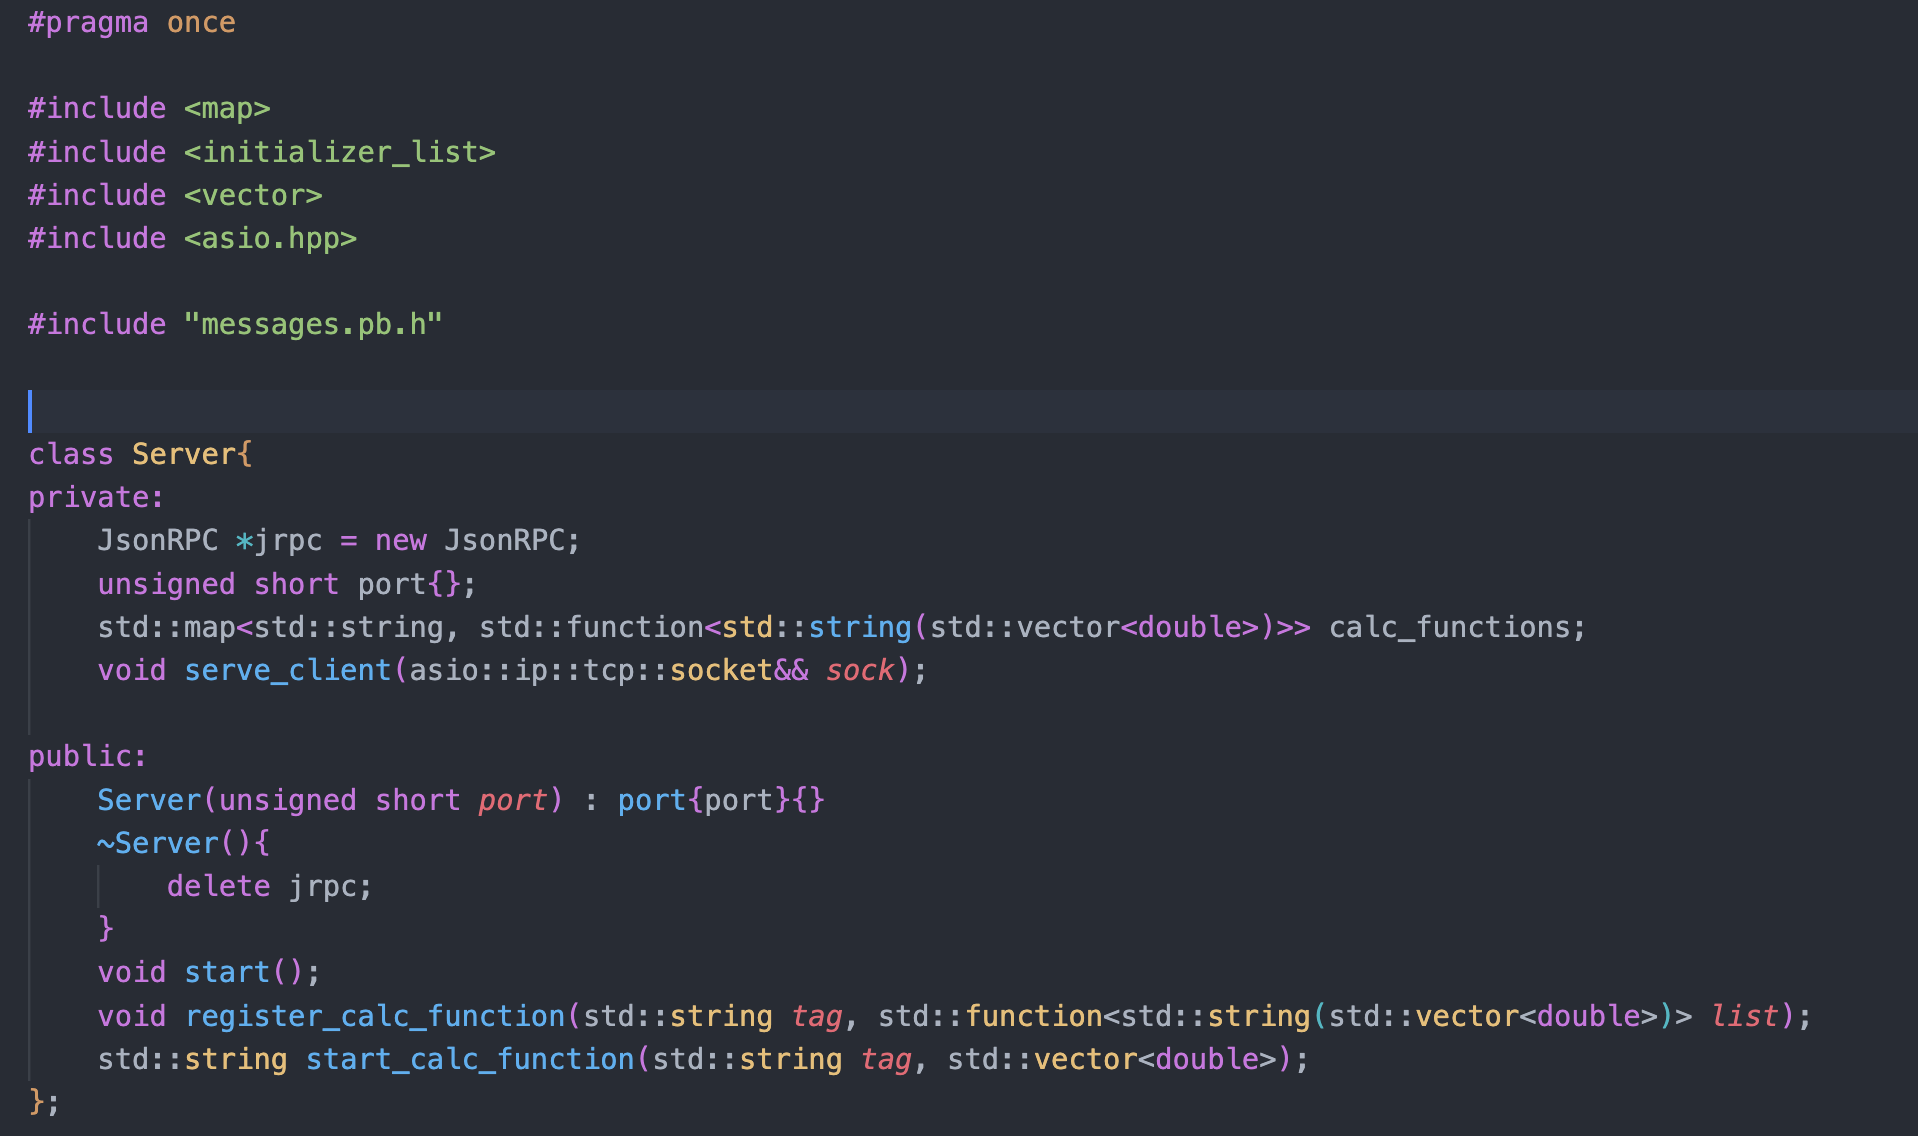
\includegraphics[width=1\textwidth]{images/Server_class.png}
  \caption{Server Klasse}
  \label{Server_h}
\end{figure}    

Für die Server-Komponente wurde der Server als eigene Klasse implementiert. Diese Klasse enthält sowohl ein JsonRPC-Objekt, welches von protobuf generiert wird, als auch die Funktionalität, neue funcitonen mit einem ''Tag'' zu registrieren und auszuführen.
\newpage
Die registrierten Funktionen werden in einer map gespeichert. In dieser map wird der ''Tag'' als Schlüssel verwendet um die Funktionen eindeutig zu identifizieren. Als Schlüssel wird dann ein Funktionspointer gespeichert. 
\begin{figure}[h!]
  \centering
  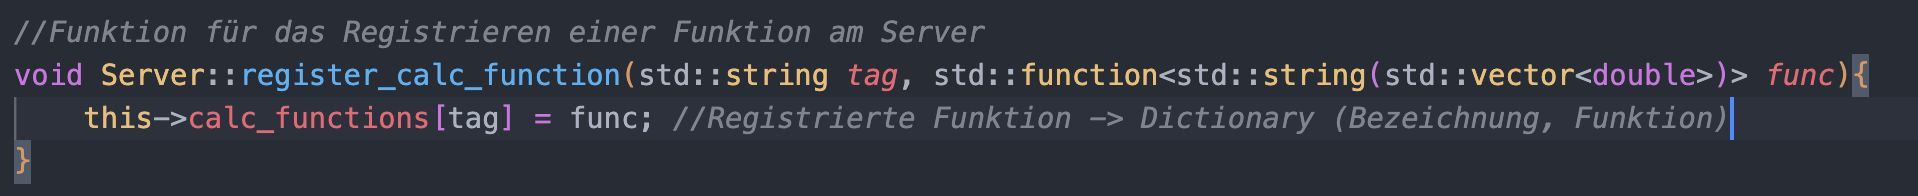
\includegraphics[width=1\textwidth]{images/Server_register.png}
  \caption{Server Register Function}
  \label{Server_register}
\end{figure}    
Die Funktion ''register\_calc\_function'' wird verwendet um neue Funktionen mit einem ''Tag'' in der map abzulegen. 
\\
\\
\begin{figure}[h!]
  \centering
  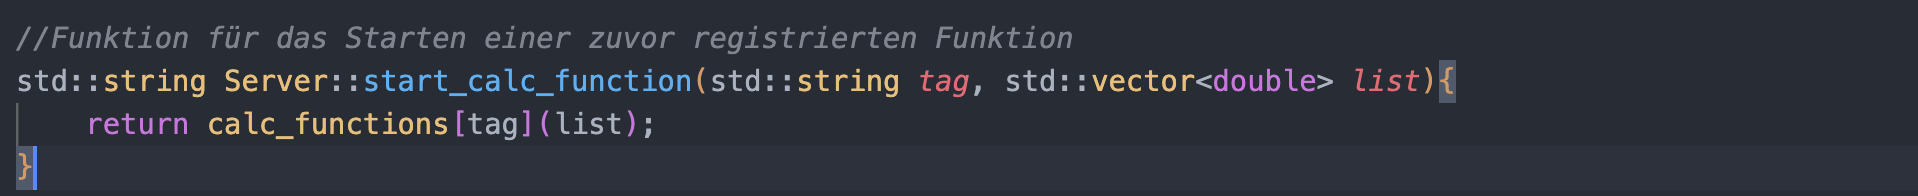
\includegraphics[width=1\textwidth]{images/Server_start_registered.png}
  \caption{Server start function}
  \label{Server_start_registered}
\end{figure}    
\\
Die Fuktion ''start\_calc\_function'' started dann die registrierte Funktion mit dem übergeben ''Tag'' und den, in einem vector übergebenen, parametern.
\\
\\
\begin{figure}[h!]
  \centering
  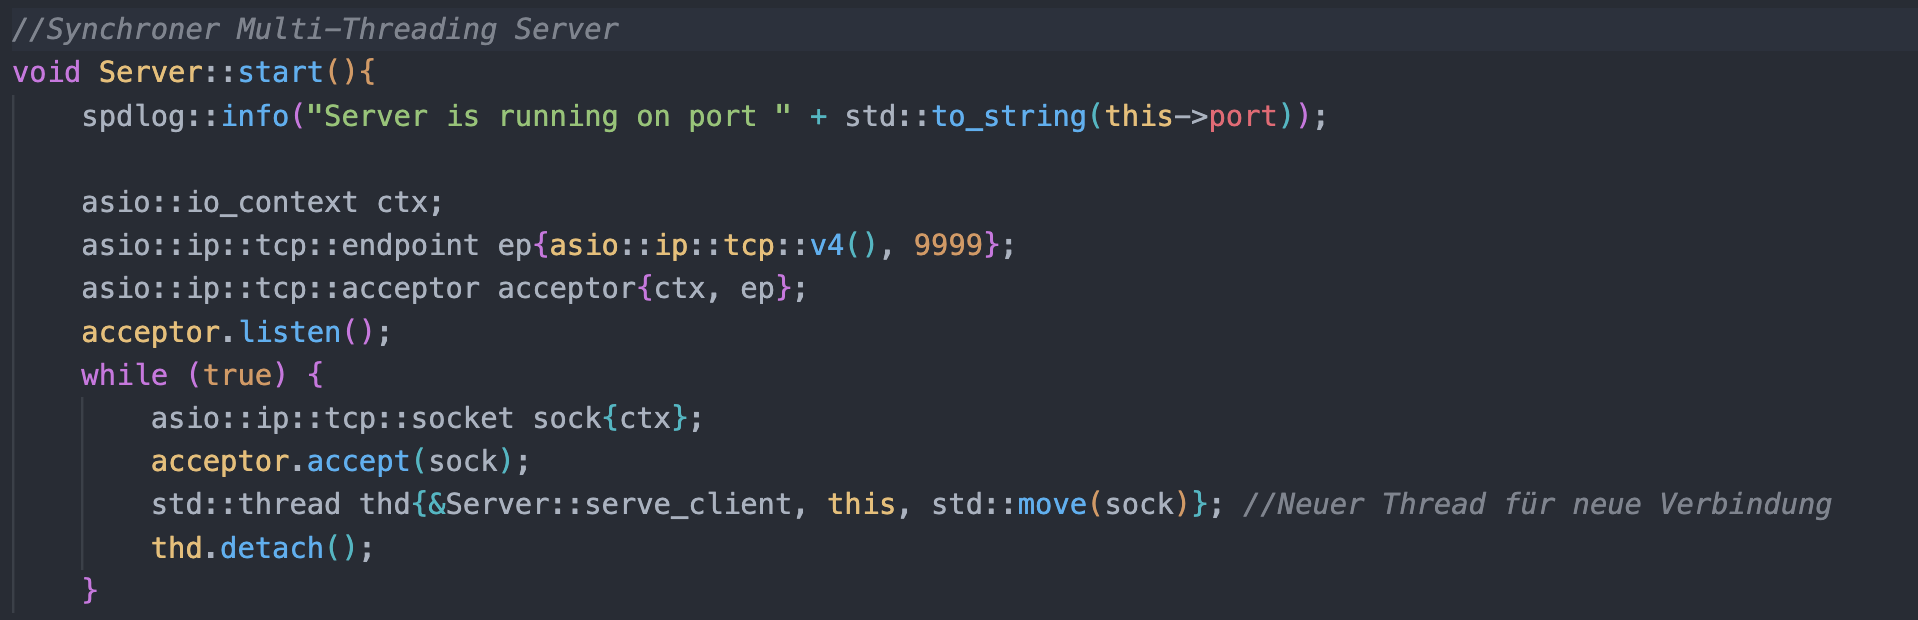
\includegraphics[width=1\textwidth]{images/Server_start.png}
  \caption{Server Start-Funktion}
  \label{Server_start}
\end{figure}    
\\
Die Funktion ''start()'' started den Server und versetzt ihn in einen Zustand in dem er Verbindungen von einem oder mehreren Cients annimmt. Wenn er eine Verbindung über einen Socket annimmt, started der Server einen neuen Thread, welcher mit der Aufgabe, die Anfrage des Clients zu bearbeiten, beauftragt wird. 
\\
\\
\newpage
\begin{figure}[h!]
  \centering
  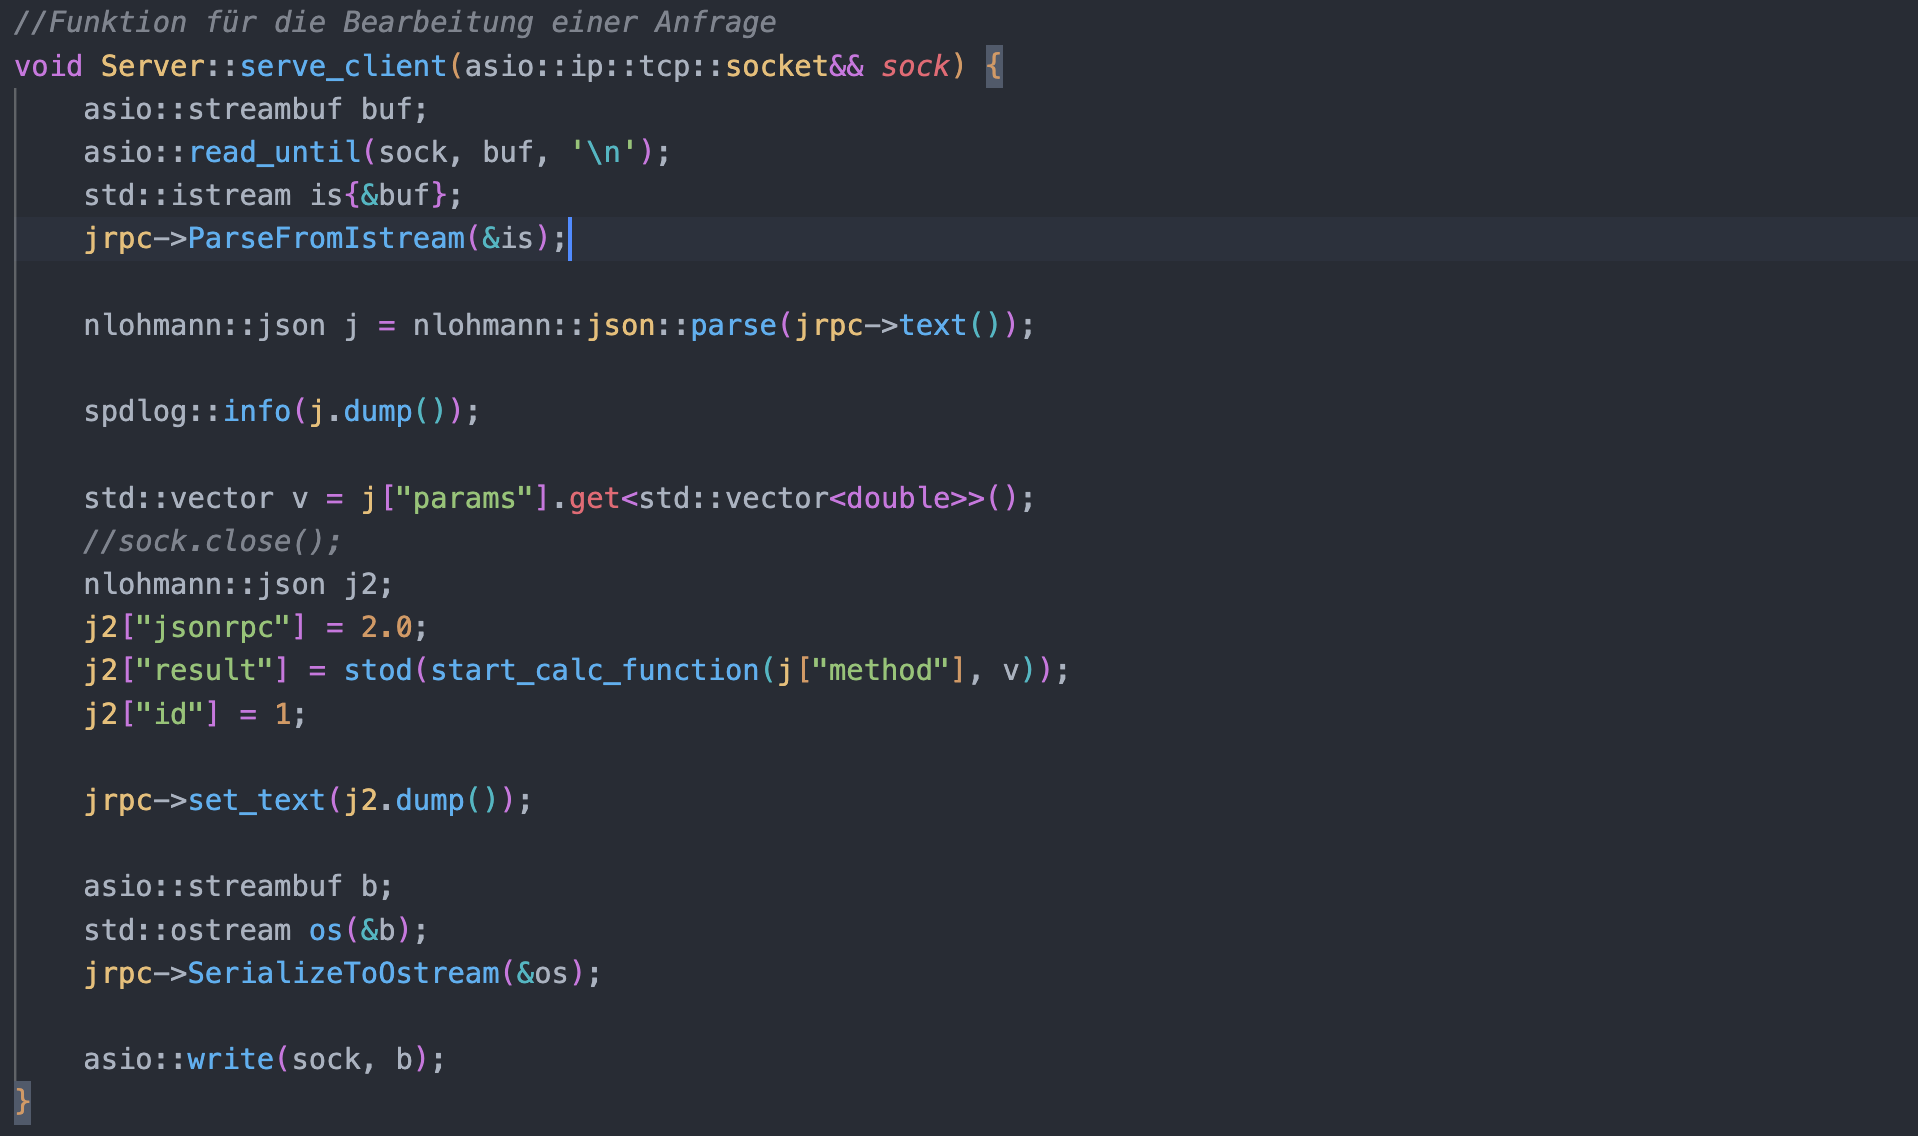
\includegraphics[width=1\textwidth]{images/Server_serve.png}
  \caption{Server Serve-Client-Funktion}
  \label{Server_serve}
\end{figure}    
Die ''client\_serve'' Funktion übernimmt den Socket, welcher mit dem Client verbunden ist, als rvalue-Referenz, und bearbeitet die Anfrage des Clients. Die Funktion liest die JSON-RPC-Anfrage aus und startet die zum Tag gehörige Funktion mit den übergebenen Parametern. Nachdem die aufgerufenen Funktion am Server fertig ist wird das Ergebnis wieder in ein JSON-RPC konformes JSON-Objekt gespeichert. Dieses Objekt wird als letztes dann wieder zum Client zurückgessendet.

\subsection{Client}
\begin{figure}[h!]
  \centering
  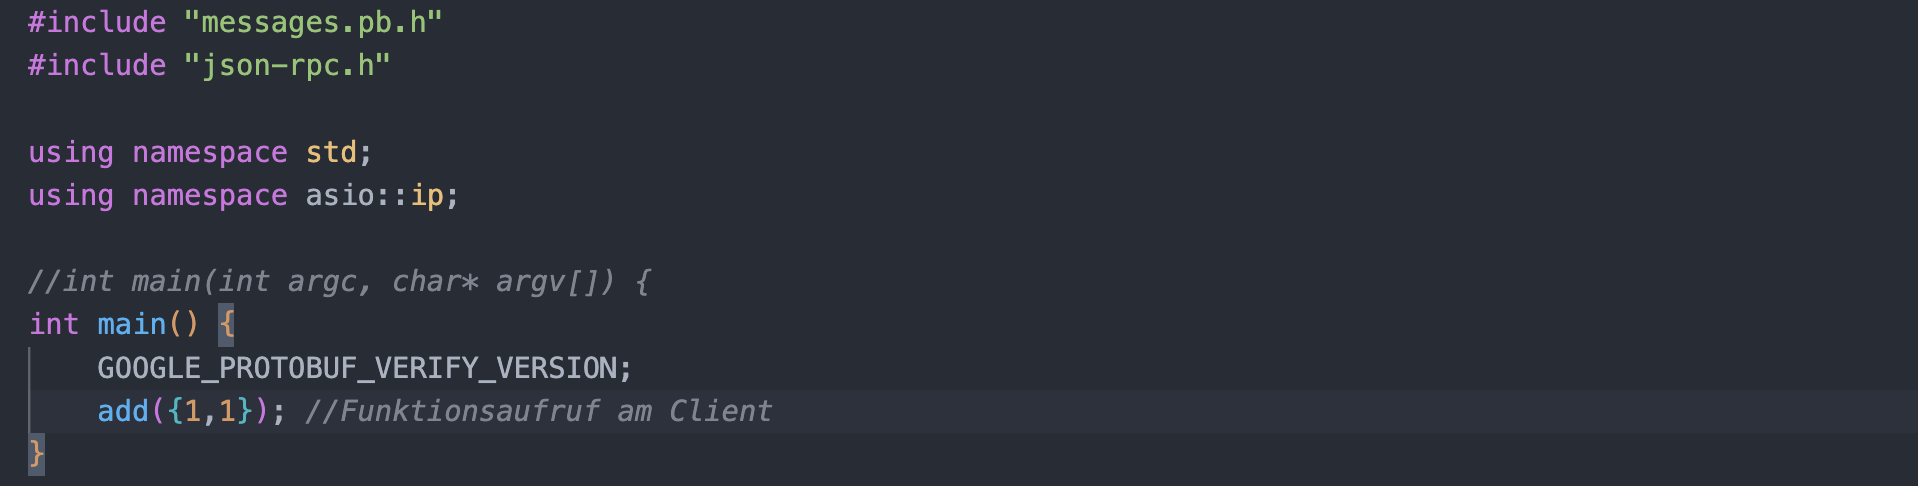
\includegraphics[width=1\textwidth]{images/Client_main.png}
  \caption{Client Main-Funktion}
  \label{Client_main}
\end{figure}    

In der main-Funktion im Client wird nur eine add Funktion mit einem Vector von Zahlen zum Addieren gestartet. In der main-Funktion kann man nicht sehen, dass die tatsächliche Berechnung nicht innerhalb des eigenen Programms abgearbeitet wird.
\\
\newpage
\begin{figure}[h!]
  \centering
  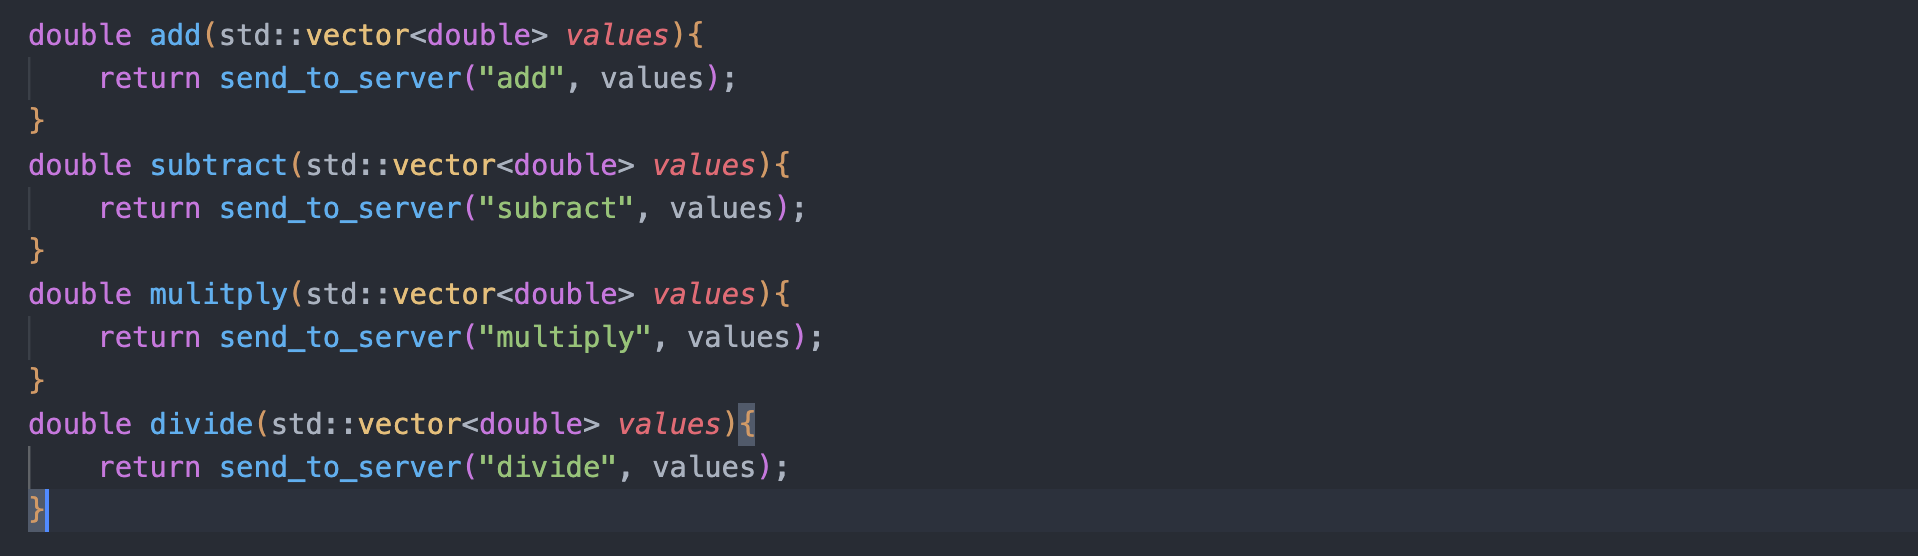
\includegraphics[width=1\textwidth]{images/Client_functions.png}
  \caption{Client Funktionen}
  \label{Client_functions}
\end{figure}   

Die Funktionen, welche von der main-Funktion am Client aufgerufen werden können, rufen alle die ''send\_to\_server()'' Funktion mit dem eigenen Funktionsnamen und einem vector von Parametern auf. 
\\
\begin{figure}[h!]
  \centering
  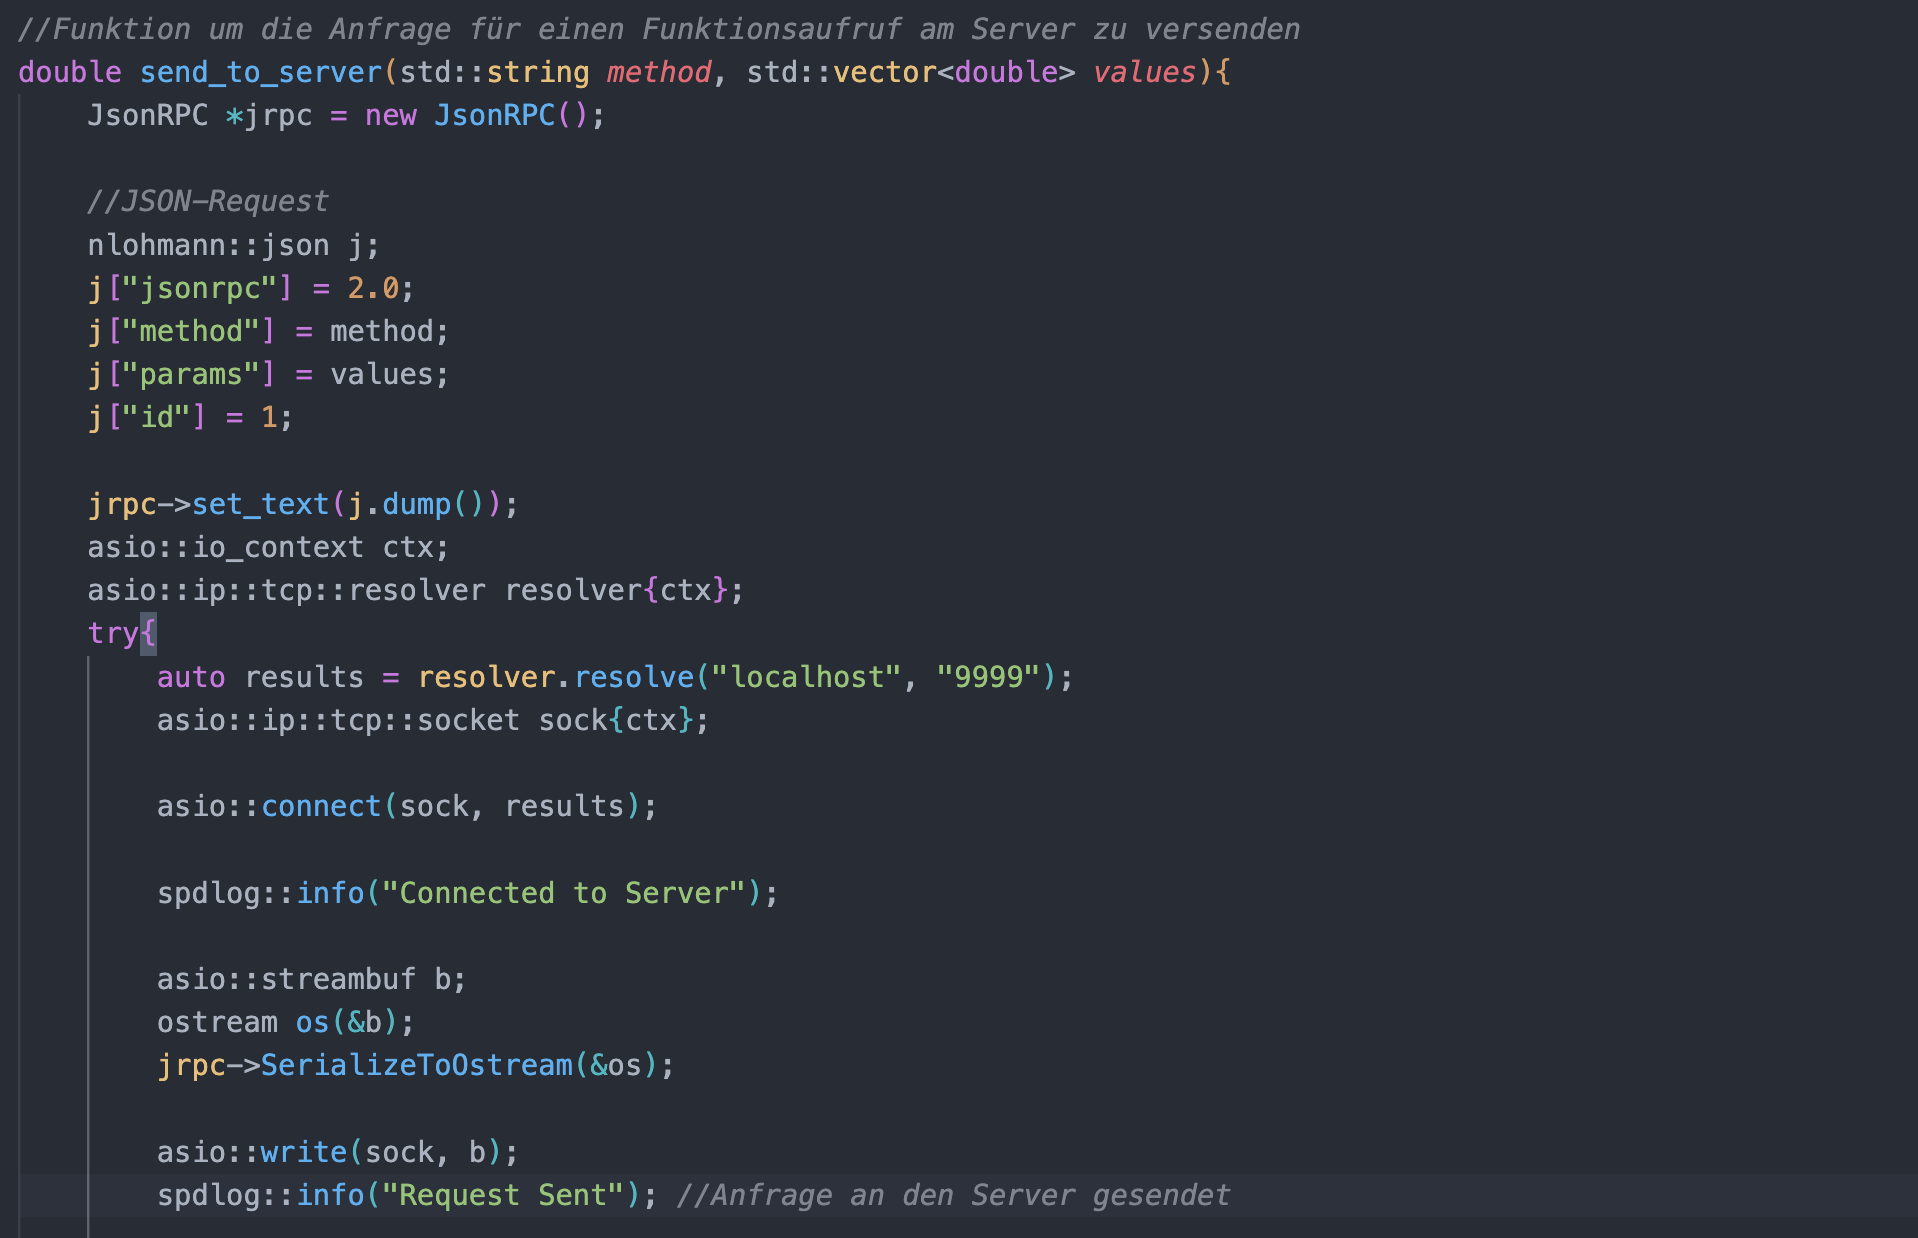
\includegraphics[width=1\textwidth]{images/Client_send.png}
  \caption{Client Send-Funktion}
  \label{Client_main}
\end{figure}   
\\
Die ''send\_to\_server''-Funktion erstellt ein neues Json-Objekt und fügt die für JSON-RPC notwendigen Parateter ein. Es werden die JSON-RPC-Version, die Methode, die Parameter und eine Id übergeben. Da die Parameter über einen vector übergeben werden, kann die verwendete json-Bibliothek die Parameter automatisch in eine Liste einfügen. Nach dem Erstellen des Json-Objekts wird eine Verbindung zum Server aufgebaut. Über  diese Verbindung wird dann der Json-String mithilfe von protobuf versendet. 
\\
\newpage
\begin{figure}[h!]
  \centering
  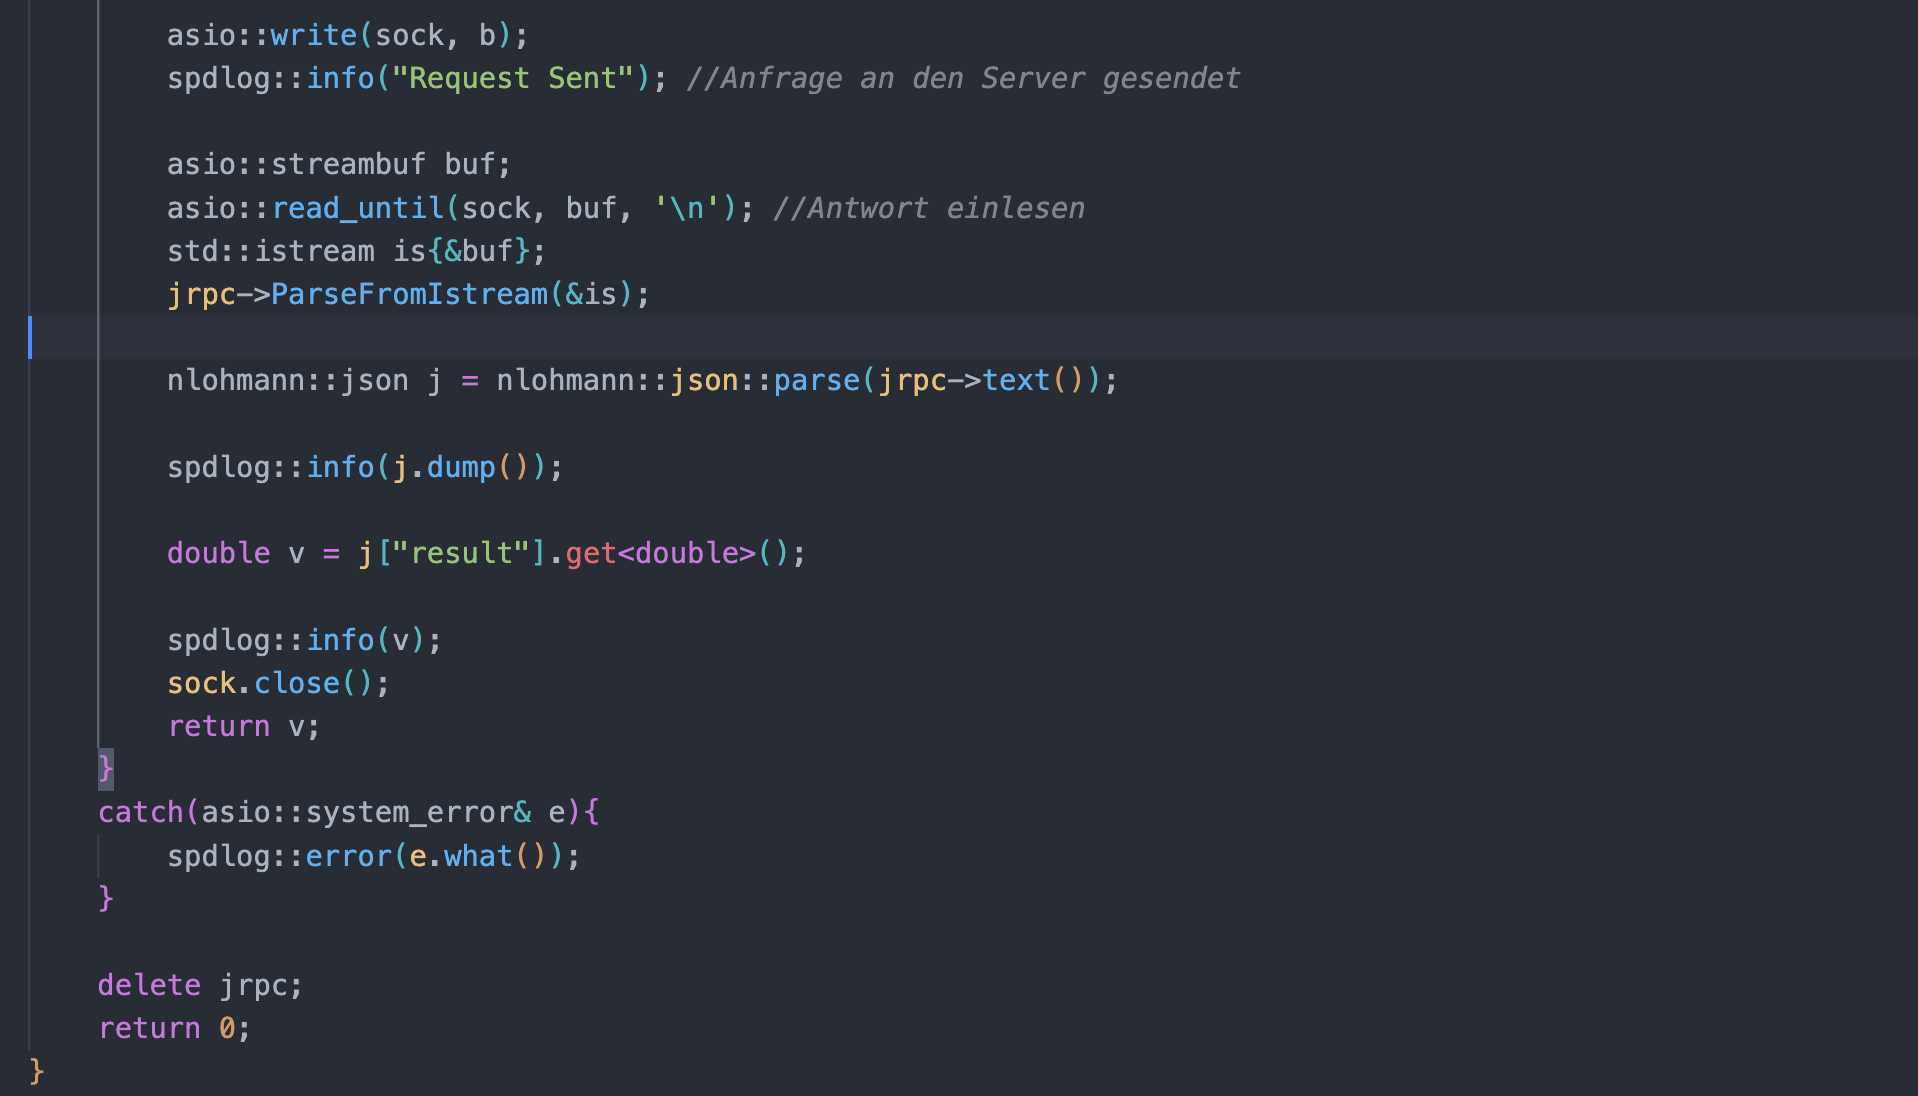
\includegraphics[width=1\textwidth]{images/Client_receive.png}
  \caption{Client Send-Funktion 2}
  \label{Cient_receive}
\end{figure}   
Nach dem Absenden des Json-Objekts über protobuf, wird auf eine Antwort vom Server gewartet. Diese Antwort wird, sobald sie ankommt, wieder zu einem Json-Objekt umgewandelt, woraus das Ergebnis ausgelesen wird. Dieses Ergebnis wird zu einem ''double' umgewandelt'. Am Ende wird dann das als ''double'' vorliegende Ergebnis zurückgeliefert, wodurch dann die main-Funktion am Client mit dem Ergebnis weiterarbeiten kann.

\chapter{Schluss}
Obwohl JSON-RPC als Protokoll viele Vorteile bietet, gibt es auch einige Nachteile, die bei der Implementierung berücksichtigt werden müssen:
\\
\\
\begin{enumerate}
    \item Keine Standardisierung von Fehlern: JSON-RPC bietet keine standardisierte Methode, um Fehler zu beschreiben, die während der Ausführung von Methoden auf dem Server auftreten können. Es liegt an den Entwicklern, eigene Fehlerbehandlungsmechanismen zu implementieren und ihre eigenen Fehlercodes zu definieren.
    \item Einschränkungen bei der Typunterstützung: JSON-RPC unterstützt nur grundlegende Datentypen wie Strings, Zahlen und Booleans sowie komplexe Datentypen wie Objekte und Arrays. Dies kann bei der Übertragung von komplexeren Datenstrukturen oder binären Daten ein Hindernis darstellen.
    \item Keine Unterstützung für Batch-Anfragen: JSON-RPC unterstützt keine Batch-Anfragen, bei denen mehrere Methoden in einer Anfrage gruppiert und gemeinsam ausgeführt werden können. Jede Anfrage muss separat gesendet werden, was zu einem erhöhten Netzwerkverkehr und einer geringeren Leistung führen kann.
    \item Keine integrierte Authentifizierung oder Verschlüsselung: JSON-RPC bietet keine integrierte Authentifizierung oder Verschlüsselung, was bedeutet, dass diese Mechanismen von den Entwicklern selbst implementiert werden müssen.
    \item Begrenzte Interoperabilität: JSON-RPC ist nicht so weit verbreitet wie andere RPC-Protokolle wie SOAP und REST, was bedeutet, dass es möglicherweise nicht von allen Client- und Serveranwendungen unterstützt wird.
\end{enumerate}
\\
\\
Insgesamt sind dies wichtige Faktoren, die bei der Implementierung von JSON-RPC berücksichtigt werden sollten, um sicherzustellen, dass das Protokoll effektiv und sicher genutzt werden kann.
\end{document}
